\section {Introduction to the analysis}

In this note, we present initial results of the tracker DAQ commissioning.
\section{Description of teststand setup}
  The tracker teststand, called TS1, included one DRAC card and one DTC connected to the DAQ computer, 96 channels in total.
The ROC could be operated in two different data readout modes: the first with
emulated data readout mode (we call it mode one) and the reading digi FPGA
readout mode (called mode two). We were operating in the mode two and the
 digi FPGAs were pulsed by the internal pulser.
  The pulser has two different frequencies,  31.29 MHz/(2$^7$+1), or approximately 250 kHz, 
and 31.29 MHz/(2$^9$+1), or approximately 60 kHz.
Event window is the time interval between two heartbeats (HB).
HB is simulated by the artdaq. 
Pulses that fall within the event window are represented in gray triangles in Fig.\ref{fig:3} and 
they are separated by the inverse of the generator frequency. We call $T_{gen}=1/f_{gen}$.
The event window, called $T_{EW}$, that simulates the distance between the proton pulses, 
could be varied from 700 ns to 50 $\mu$s.
The ROC firmware has an internal hit buffer which stores up to 255 hits.
That should be sufficient for the data taking.
Testing therefore could proceed in two different modes:
  \begin{itemize}
  \item
    The event window is large enough , so the total number of generated hits is greater than 255. In this case
    the ROC hit buffer always gets filled up, and only the first 255 hits are read out;
  \item
    The total number of hits within the event window is less than 255.
    In this case the ROC hit buffer doesn't get filled up and the total number of hits can vary from one event to another.
  \end{itemize}
The time offset between generator pulses and the start of the event window
is random (flat distribution) and because of this different number of hits 
can fit in the event window.
Due to the fact that each FPGA has its own completely random generator, there are FPGA to FPGA offsets
and these are of the order of nanoseconds.
There are also channel to channel offsets and these are three orders of magnitude less than the FPGAs ones.
Readout sequence is defined: all channels are read as the order we expect that is fixed.

\begin{figure}[!h]
\centering
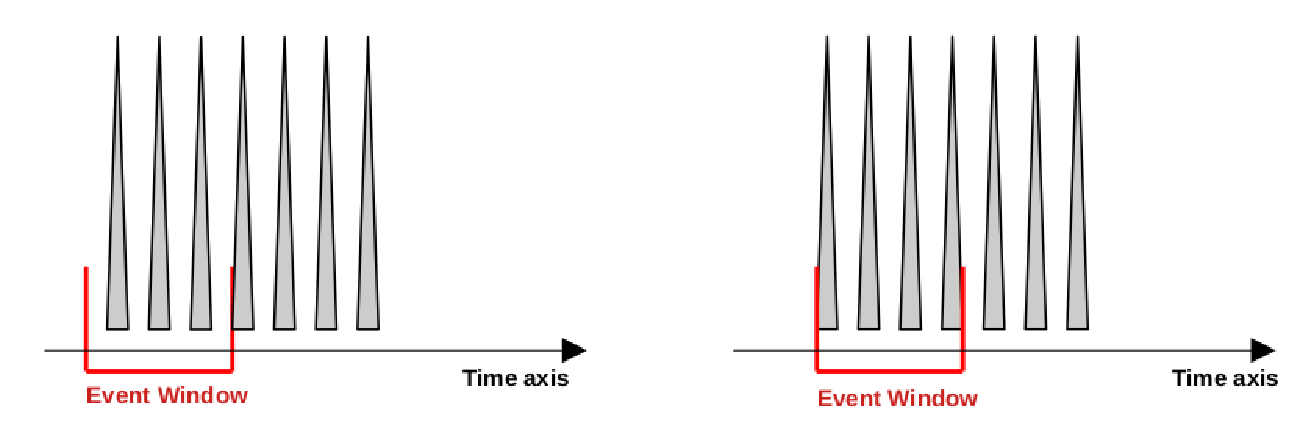
\includegraphics[width =0.8\textwidth]{figures/pdf/eventwindow}
\caption{Graphic illustration of pulses in an event window.}
\label{fig:3}
\end{figure}
\section{Monte Carlo simulation}\label{MonteCarlo}
 
As the ROC readout logic is purely digital, the readout process can be simulated.
The channel number and its hits are parameters that can be simulated, and so the occupancy (number of hits versus channel).
Given that the maximum allowable number of hits per event is 255, the simulation follows these steps:
\begin{itemize}
  \item The first pulse is generated randomly by following a uniform distribution;
    \item The following pulses are generated subtracting from the first one a step of $T_{gen}$, until the time difference between the 
first the last one is greater than $T_{EW}$;
  \item The process of pulse creation continued until the count of hits reached the maximum threshold of 255,
 at which point the event construction is terminated. This determines the number of hits for each channel.
\end{itemize}
This operation is performed for all channels.
Furthermore, the simulation accounts for the channel to channel and FPGA to FPGA offsets. 


%%% Local Variables:
%%% mode: latex
%%% TeX-master: t
%%% End:

